% !TeX root = ../sustechthesis-example.tex

\chapter{气体动理论}


\section{理想气体}


\section{速度分布函数与宏观量}\label{sec:Boltzmann}

在气体动理论中,单原子气体在相空间中的概率密度由速度分布函数$f(t,\bm{x},\bm{v})$表示,是时间$t$, 空间坐标$ \bm{x}=(x_1,x_2,x_3)$ 和 分子速度$\bm{v}=(v_1,v_2,v_3)$的函数. 定义$f(t,\bm{x},\bm{v})d\bm{x}d\bm{v}$是体积为$d\bm{x}d\bm{v}$的相空间上的分子数,则气体的数密度$n$、宏观速度$\bm{u}$、温度$T$、压力张量$p_{ij}$和热流$\bm{q}$可以分别通过对速度分布函数求矩得到:
\begin{equation}\label{macroscopic_origin}
\begin{aligned}[b]
&n(t,\bm{x})=\int{}f(t,\bm{x},\bm{v})d\bm{v}, \\  &\bm{u}(t,\bm{x})=\frac{1}{n(t,\bm{x})}\int\bm{v}f(t,\bm{x},\bm{v})d\bm{v},\\   &T(t,\bm{x})=\frac{m}{3k_Bn(t,\bm{x})}\int{}c^2f(t,\bm{x},\bm{v})d\bm{v}, \\    &p_{ij}(t,\bm{x})={}m\int{}c_ic_jf(t,\bm{x},\bm{v})d\bm{v}, \\  &\bm{q}(t,\bm{x})=\frac{m}{2}\int{}c^2\bm{c}f(t,\bm{x},\bm{v})d\bm{v},
\end{aligned}
\end{equation}
其中, $\bm{c}=\bm{v}-\bm{u}$是气体分子热运动速度, 即气体分子速度与当地宏观速度的矢量差,而$c$是热运动速率. 定义应力偏量为
\begin{equation}
\sigma_{ij}=p_{ij}-p\delta_{ij},
\end{equation}
其中$p=nk_BT$, $\delta_{ij}$为克罗内克函数. 


\section{Boltzmann方程}

The governing equation for the evolution of VDF of a dilute gas system is derived by Ludwig Boltzmann. In his description, molecules move in straight lines with fixed velocities until they encounter elastic collisions with other molecules. This is justified by the fact that, at standard temperature and pressure, the MFP of gas molecules is hundreds times of the nominal atomic diameter and about 30 times the average molecular separation.  

Both molecular streaming and collision change the VDF in the phase space as per the Boltzmann equation~\cite{CE,Cercignani1990,henning,Kremer2009book}:
\begin{equation}\label{Boltzmann}
\frac{\partial f}{\partial t}+\bm{v}\cdot\frac{\partial f}{\partial
	\bm{x}}+\bm{a}\cdot\frac{\partial f}{\partial \bm{v}}={Q(f,f_*)},
\end{equation}
where the first term on the left hand side describes the change of VDF with respect to time, the second term is the convective change, and the third term represents the change of VDF induced by external acceleration (suppose it is independent of the molecular velocity). They together describe the streaming of gas molecules. 

The quadratic collision operator $Q(f,f_*)$ describes the change of molecular numbers per unit phase-space volume $d\bm{x}d\bm{v}$ and per unit time. This change consists of two effects. First, when the molecule with velocity $\bm{v}$ collides with another molecule with velocity $\bm{v}_\ast$, its velocity becomes $\bm{v}'$, which contributes to the loss of  molecules with the very velocity $\bm{v}$. During time interval $\Delta{t}$, there are 
\begin{equation}\label{total_collision}
f(t,\bm{x},\bm{v}_\ast)v_r\Delta{t}bdbd\phi{}d\bm{v}_\ast
\end{equation}
such collisions. Therefore, the number of molecule lost in the binary collision per unit phase-space volume and per time is
\begin{equation}
\begin{aligned}[b]
Q_{\text{loss}}&=\frac{\int{}f(t,\bm{x},\bm{v})d\bm{x}d\bm{v}\times
	f(t,\bm{x},\bm{v}_\ast)v_r\Delta{t}bdbd\phi{}d\bm{v}_\ast}{d\bm{x}d\bm{v}\Delta{t}}\\
&=\frac{\int{}f(t,\bm{x},\bm{v})d\bm{x}d\bm{v}\times
	f(t,\bm{x},\bm{v}_\ast)v_r\Delta{t}
	\sigma_D\sin\theta{d\theta}d\phi{}d\bm{v}_\ast}{d\bm{x}d\bm{v}\Delta{t}}\\
&=\int_{\mathbb{R}^3}\int_{\mathbb{S}^{2}}
B(\cos\theta,v_r)
f(t,\bm{x},\bm{v}_{\ast})f(t,\bm{x},\bm{v})
d\Omega
d\bm{v}_\ast.
\end{aligned}
\end{equation}
Second, when the molecule with velocity $\bm{v}'$ collides with another molecule with the velocity $\bm{v}'_\ast$, its velocity becomes $\bm{v}$, which contributes to the gain of molecules with the very velocity $\bm{v}$. Therefore, with the facts that $d\bm{v}d\bm{v}_\ast=d\bm{v}'d\bm{v}'_\ast$, $v_r=v'_r$, and the collision kernel is only determined by the relative collision speed and impact parameter, the gain part of the Boltzmann collision operator is
\begin{equation}
\begin{aligned}[b]
Q_{\text{gain}}&=\frac{\int{}f(t,\bm{x},\bm{v}')d\bm{x}d\bm{v}'\times
	f(t,\bm{x},\bm{v}'_\ast)v'_r\Delta{t}bdbd\phi{}d\bm{v}'_\ast}{d\bm{x}d\bm{v}\Delta{t}}\\
&=\int_{\mathbb{R}^3}\int_{\mathbb{S}^{2}}
B(\cos\theta,v_r)
f(t,\bm{x},\bm{v}'_{\ast})f(t,\bm{x},\bm{v}')
d\Omega
d\bm{v}_\ast.
\end{aligned}
\end{equation}
Finally, the Boltzmann collision operator \index{Boltzmann collision operator} is written in the following form (since it is local in time and space, for simplicity $t$ and $\bm{x}$ will be omitted in writing the collision operator):
\begin{eqnarray}\label{chapter1_collision}
Q(f,f_*)=\int_{\mathbb{R}^3}\int_{\mathbb{S}^{2}}
B(\cos\theta,v_r)
[f(\bm{v}'_{\ast})f(\bm{v}')-
f(\bm{v}_{\ast})f(\bm{v})]
d\Omega
d\bm{v}_\ast.
\end{eqnarray}
Note that the ``Stosszahlansatz'' or assumption of molecular chaos was used implicitly, that is, the value of VDF for different velocities are independent. 

%

%The Boltzmann equation is more complicated than the NSF equations, not only because the VDF is defined in six-dimensional phase-space (three dimensional spatial space and three dimensional velocity space), but also because of its high dimensional collision operator (fivefold integral with three dimensions in velocity space and two dimensions in a unit sphere). Therefore, it is highly desirable to have macroscopic equations like the NSF ones. To eliminate the microscopic velocity variables, moment equations from the Boltzmann equation should be considered. Multiplying Eq.~\eqref{Boltzmann} by 1, $\bm{v}$, and $|\bm{v}|^2$, and integrating the resulting equations with respect to the molecular velocity $\bm{v}$, one gets Eqs.~\eqref{macro_denstiy}--\eqref{macro_temperature}. However, these equations are not closed because expressions for shear stress and heat flux are not known. 


对于稀疏气体 ~(dilute gas,分子间距远远大于分子直径),在外部施加的加速度$\bm{a}=(a_1,a_2,a_3)$的作用下,速度分布函数的演化由玻尔兹曼方程描述:
\begin{equation}\label{Boltzmann}
\frac{\partial f}{\partial t}+\bm{v}\cdot\frac{\partial f}{\partial
	\bm{x}}+\bm{a}\cdot\frac{\partial f}{\partial \bm{v}}={Q(f)}.
\end{equation}
方程左边的三项分别表示速度分布函数在时间上的变化,在速度作用下在物理空间的变化,以及在外力作用下在速度空间的变化;右边表示使得分布函数趋于平衡态的气体分子的碰撞过程. 在玻尔兹曼方程中,二体碰撞的形式为:
\begin{equation}\label{chapter1_collision}
Q(f)=\iint{}B(\theta,{v}_r) 
[f(\bm{v}'_*)f(\bm{v}')-f(\bm{v}_*)f(\bm{v})]d{\Omega}d\bm{v}_*.
\end{equation}
其中,$\bm{v}$ 和 $\bm{v}_\ast$ 分别是碰撞前两个分子的速度,而$\bm{v}'$ 和 $\bm{v}'_\ast$是它们碰撞后的速度.  由于碰撞前后两分子的距离足够远以至于它们的相互作用可以忽略不计,根据动量和能量守恒定律,碰撞前后速度关系如下:
\begin{equation}\label{collision_velocity}
\begin{aligned}[b]
\bm{v}'&=\frac{\bm{v}+\bm{v}_\ast}{2}+\frac{|\bm{v}-\bm{v}_\ast|}{2}\Omega,\\%=\bm{v}+\frac{{v_r}\Omega-\bm{v}_r}{2}
\bm{v}'_\ast&=\frac{\bm{v}+\bm{v}_\ast}{2}-\frac{|\bm{v}-\bm{v}_\ast|}{2}\Omega.%=\bm{v}_\ast-\frac{{v_r}\Omega-\bm{v}_r}{2},
\end{aligned}
\end{equation}
碰撞的示意图见图~\ref{Boltzmann_collision_demo}. 其中,碰撞前两分子的相对速度为 $\bm{v}_r=\bm{v}-\bm{v}_\ast$,碰撞后的相对速度为 $\bm{v}'-\bm{v}'_\ast$. $\Omega$ 为定义在单位球空间的矢量,它与碰撞后的相对速度同方向. 于是相对速度的偏转角$\theta$与碰撞前相对速度满足如下关系:
\begin{equation}
\cos\theta=\Omega\cdot\frac{\bm{v}_r}{{v}_r}.
\end{equation}
最后,碰撞核$B(\theta,v_r) $是相对速度和碰撞偏转角度的函数,具体形式取决于分子间的作用力. 


\begin{figure}[t]
	\centering
	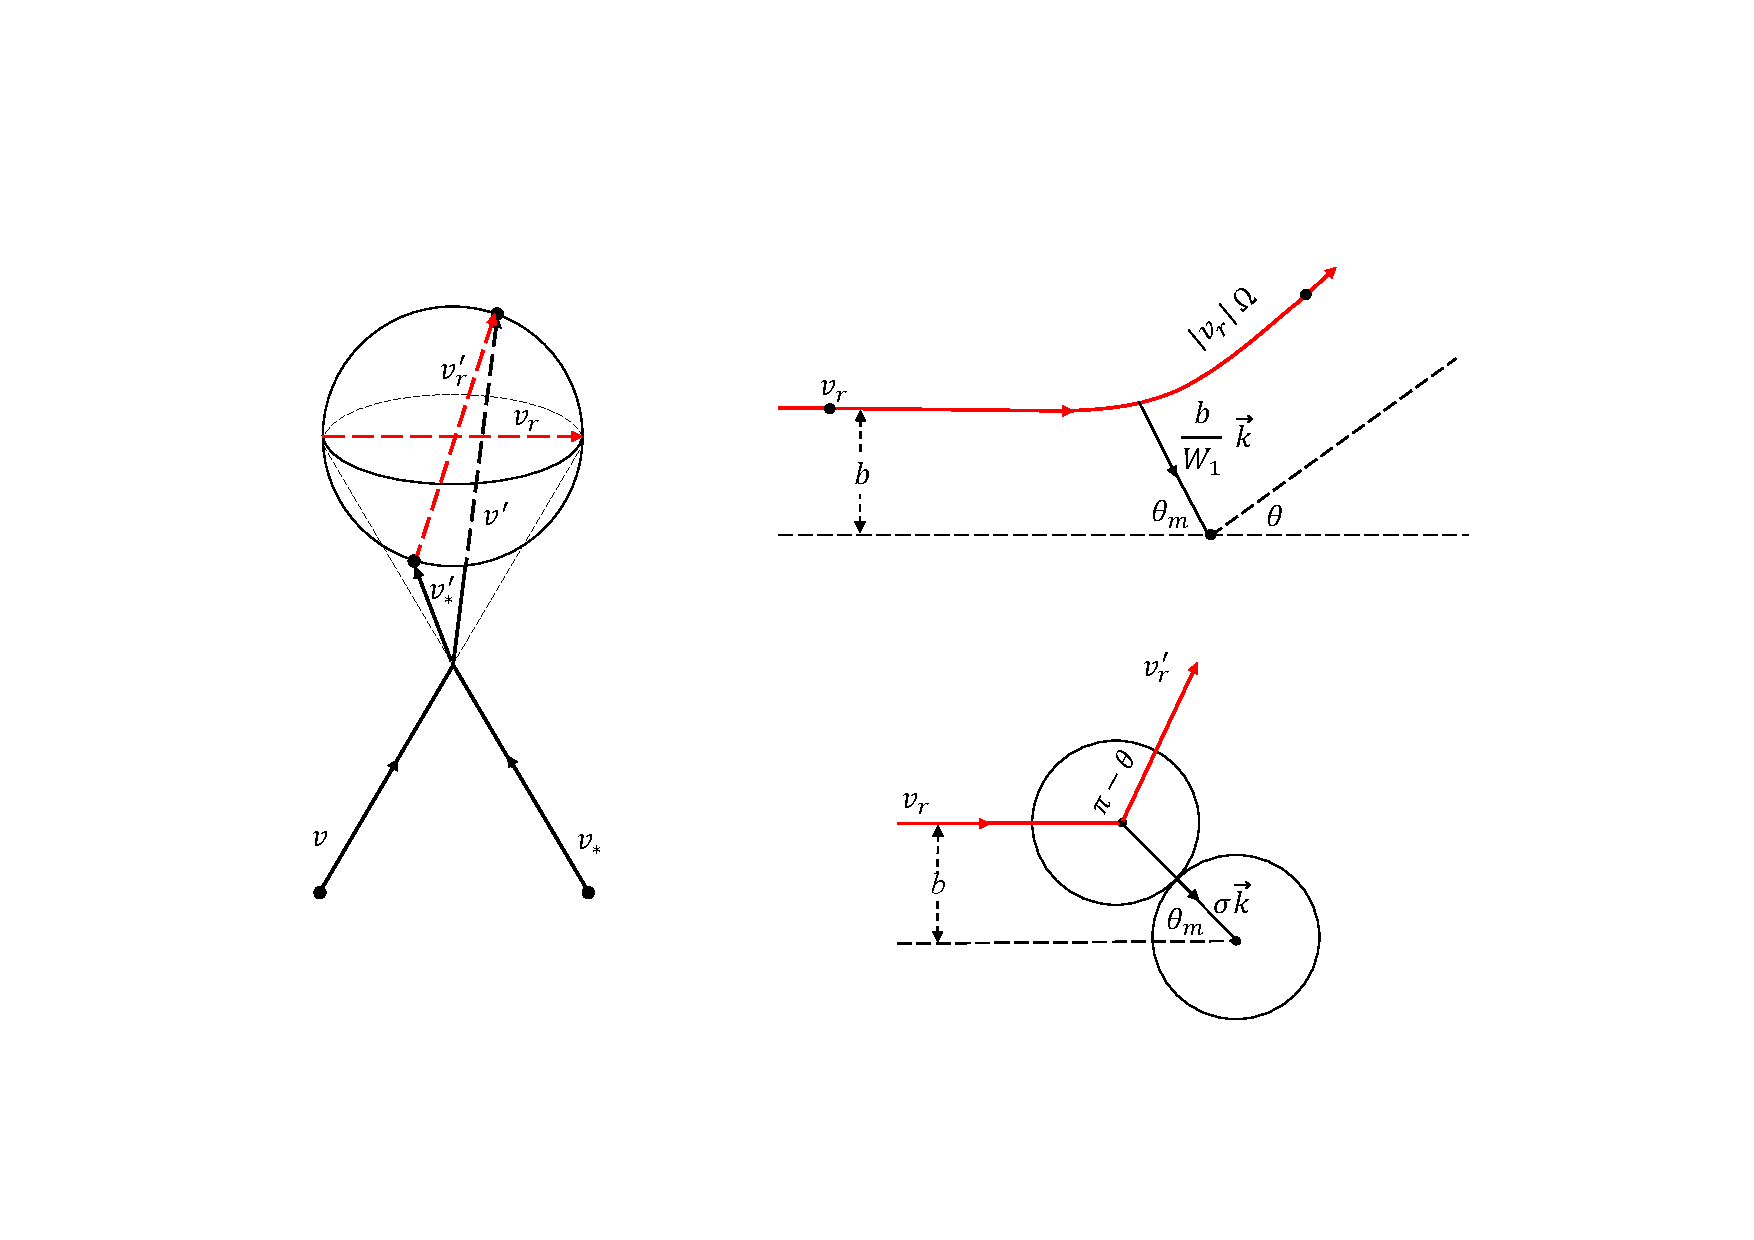
\includegraphics[width=0.9\textwidth]{Fig/Boltzmann_collision_demo.pdf}
	\caption{(左) 二体碰撞前后的速度分布. 由于动量和能量守恒,碰撞前后的相对速度分布在球体上并且通过球心.(右上)中心力场作用下的经典二体碰撞示意图,其中$b$ 为瞄准距离,$\bm{k}$ 为沿两分子间最短距离方向的单位矢量.(右下)直径为$\sigma$ 的硬球分子的两体碰撞.
	}
	\label{Boltzmann_collision_demo}
\end{figure}




\subsection{偏转角和微分散射截面}


假设分子间通过中心力场作用,作用势$\phi(r)$已知, 其中$r$为分子间距,则偏转角可以通过经典力学和量子力学两种方式求解.  若气体温度不低~(如氦气的温度高于100~K),两种方式得到的输运系数(如粘性和热导率)相同\cite{Sharipov2018Vacuum}. 这里仅介绍经典力学的计算结果,如图~\ref{Boltzmann_collision_demo}所示,偏转角可以表示为:
\begin{equation}\label{deflection}
\theta(b,{v}_r)=\pi-2\int_0^{W_1}\left[1-W^2-\frac{4\phi(r)}{m{v}_r^2}\right]^{-1/2}dW,
\end{equation}
其中,$W=b/r$为瞄准距离$b$与分子间距$r$的比值, 积分上限$W_1$对应于最短分子间距,即上式中括号内表达式等于零的方程的正根. 


%碰撞的微分散射截面为
%\begin{equation}\label{DCS_chapter1}
%\sigma_D=\frac{b|db|}{\sin\theta|d\theta|}=\left(\frac{m(\eta-1)}{4K}\right)^{2\eta-2}v^{-\frac{4}{\eta-1}}_r\times\frac{sds}{\sin\Theta{d\Theta}},
%\end{equation}
%碰撞核为
%\begin{equation}
%B(\theta,{v}_r)=v_r\sigma_D.
%\end{equation}


%although the Lennard-Jones potential is widely used (say, in the MD simulation of monatomic gas):
%\begin{equation}\label{Lennard_Jones_chapter}
%\phi(r_{ij})=4\epsilon\left[\left(\frac{d_{LJ}}{r_{ij}}\right)^{12}-\left(\frac{d_{LJ}}{r_{ij}}\right)^6\right],
%\end{equation}

%where $\epsilon$ is the potential depth and $d_{LJ}$ is the distance between two molecules where the potential is zero. 

在气体动理论中,经常考虑如下形式的逆幂律分子作用势:
\begin{equation}\label{power_law_potential}
\phi(r)=\frac{K}{\eta-1}r^{1-\eta},
\end{equation}
其中, $K$表征分子间相互作用的强度.  从公式~\eqref{deflection} 可知,偏转角只与变量$s$有关,即$\theta=\Theta(s)$:
\begin{equation}\label{impact_norm}
s=\left[\frac{m(\eta-1)}{4K}\right]^{\frac{1}{\eta-1}}bv^{\frac{2}{\eta-1}}_r.
\end{equation}

微分散射截面定义为
\begin{equation}\label{DCS_chapter1}
\begin{aligned}[b]
\sigma_D&=\frac{b|db|}{\sin\theta|d\theta|}\\
&=\left(\frac{m(\eta-1)}{4K}\right)^{\frac{2}{1-\eta}}v^{\frac{4}{1-\eta}}_r
\frac{sds}{\sin\Theta{d\Theta}},
\end{aligned}
\end{equation}
而碰撞核为
\begin{equation}
B(\theta,v_r)=v_r \sigma_D.
\end{equation}


当公式\eqref{power_law_potential}中$\eta=5$时,即为麦克斯韦分子,此时碰撞核与相对碰撞速度无关,记为 $B(\theta,v_r)=\sqrt{2K/m}B(\theta)$. 
对于硬球分子模型,可看作式\eqref{power_law_potential}中$\eta=\infty $,从图~\ref{Boltzmann_collision_demo}可以看出,偏转角可通过如下公式确定:
$b=\sigma\cos\left({\theta}/{2}\right)$,其中$\sigma$为硬球直径. 因此微分散射截面为 $\sigma_D={{\sigma}^2}/{4}$,而碰撞核为 $B(\theta,{v}_r)={\sigma}^2v_r/4$.  对于一般的气体,它们的行为介于麦克斯韦分子和硬球分子之间. 




\subsection{熵增原理}


对于任意关于分子速度的函数$\Psi(\bm{v})$,对玻尔兹曼碰撞项~\eqref{chapter1_collision} 在速度空间积分,具有如下对称性:
\begin{equation}\label{symmetry_collision}
\begin{aligned}[b]
\int\Psi(\bm{v})Q(\bm{v})d\bm{v}=&\frac{1}{4}\iiint d\Omega
d\bm{v}_\ast{d\bm{v}}
\Delta[\Psi]
B(\theta,v_r)\\
&\times \left[f(\bm{v}'_{\ast})f(\bm{v}')-f(\bm{v}_{\ast})f(\bm{v})\right],
\end{aligned}
\end{equation}
其中
$\Delta[\Psi]=
\Psi(\bm{v}_{\ast})+\Psi(\bm{v})
-\Psi(\bm{v}'_{\ast})-\Psi(\bm{v}')$. 
若$\Psi$满足 $\int\Psi(\bm{v})Qd\bm{v}=0$,则称其为碰撞不变量. 根据质量、动量和能量守恒,可知 $\Psi=1,\bm{v}, v^2$ 为碰撞不变量,而碰撞不变量的线性组合也是碰撞不变量. 

定义 $H$ 函数为:
\begin{equation}\label{entropy_function}
H=-\iint {f\ln}fd\bm{v}d\bm{x},
\end{equation}
是与气体系统的熵相关的标量.  在无外力的情况下,$H$ 的时间导数可写为:
\begin{equation*}
\begin{aligned}[b]
\frac{\partial H}{\partial t}=&	-\iint(1+{\ln}f)\frac{\partial{f}}{\partial{t}}d\bm{v}d\bm{x}\\
=&\iint{\bm{v}\cdot\frac{\partial{f}\ln{f}}{\partial\bm{x}}}d\bm{v}d\bm{x}-\iint(1+\ln{f}){Q} d\bm{v}d\bm{x}\\
=&\oint \int{\bm{v}\cdot\bm{n} {f}\ln{f}}d\bm{v}dS-\iint(1+\ln{f}){Q} d\bm{v}d\bm{x}.
\end{aligned}
\end{equation*}
式中,$\bm{n}$ 为系统表面微元 $dS$ 的外法线.  对于孤立系统,上式右端第一项为零;利用方程~\eqref{symmetry_collision},右端项第二项可写为:
\begin{equation*}
\begin{aligned}[b]
\frac{1}{4}\iiint{}&d\Omega
d\bm{v}_\ast{d\bm{v}}
B
\left[f(\bm{v}'_{\ast})f(\bm{v}')-f(\bm{v}_{\ast})f(\bm{v})\right]\\
&\times
\left\{
\ln[f(\bm{v}'_{\ast})f(\bm{v}')]
-\ln[f(\bm{v}_{\ast})f(\bm{v})]
\right\}.
\end{aligned}
\end{equation*}
因为碰撞核$B$非负,且对于任意的两个正整数 $a$ 和 $b$,不等式 $(a-b)(\ln{a}-\ln{b})\ge0$ 恒成立, 所以有
\begin{equation}\label{entropy_inequality}
\frac{\partial H}{\partial t}\ge0.
\end{equation}

上式表明孤立系统的$H$函数不会减小,这就是著名的玻尔兹曼的熵增原理. $H$随时间单调增加,但存在有限的上界,上界对应为式~\eqref{entropy_inequality}中等号成立时的平衡态, 即
$\ln{f}(\bm{v}_{\ast})+\ln{f}(\bm{v})
=\ln{f}(\bm{v}'_{\ast})+\ln{f}(\bm{v}')$. 
因此,$\ln{f}$ 也是碰撞不变量,可以表示为五个基本碰撞不变量 的线性组合:
$\ln{f}=\alpha_1+\bm{\alpha}_2\cdot\bm{v}+\alpha_3v^2$;给定系统的密度、速度和温度,
参数$\alpha_1$, $\alpha_3$ 和$\alpha_2$ 可以唯一确定. 此时,麦克斯韦平衡态速度分布函数为
\begin{equation}\label{equilibrium_Maxwellian}
F_{eq}(T)=n\left(\frac{m}{2\pi   k_BT}\right)^{3/2}\exp\left(-\frac{mc^2}{2k_BT}\right).
\end{equation}


\subsection{线性化玻尔兹曼方程}\label{LBE_chapter1}

线性化玻尔兹曼方程在气体动理论中具有重要地位. 第一,线性化玻尔兹曼碰撞项的本征值与本征函数,不仅在渐近展开推导纳维-斯托克斯方程的过程中至关重要,而且是发展简化动理学模型方程的源头理论. 第二,在许多微机电系统中,气体的压力梯度与温度梯度非常小,因此使用线性化方程可以高效准确地模拟微流动. 第三,虽然玻尔兹曼方程是单粒子速度分布函数确定性演化的平均方程,但是在某些问题中(例如:第\ref{RBS_section}节中的瑞利-布里渊散射)可以通过线化玻尔兹曼方程研究粒子涨落带来的影响. 

通常将速度分布函数在全局平衡态
\begin{equation}
f_{eq}=n_0\left(\frac{m}{2\pi   k_BT_0}\right)^{3/2}\exp\left(-\frac{mv^2}{2k_BT_0}\right)
\end{equation}
下展开为
\begin{equation}\label{chapter_vdf_lin_origin}
f(t,\bm{x},\bm{v})=f_{eq}(\bm{v})\left[1+\phi(t,\bm{x},\bm{v})\right],
\end{equation} 
其中扰动量 $\phi$ 满足约束条件 $|\phi|\ll1$. 不考虑外力项,只保留$\phi$的一次项,玻尔兹曼方程~\eqref{Boltzmann}可线性化为如下形式:
%\begin{widetext}
\begin{equation}\label{Chapter1_Boltzmann_lin0}
\begin{aligned}[b]
\frac{\partial\phi}{\partial t}+\bm{\xi}\cdot\frac{\partial\phi}{\partial
	\bm{x}}
&=\frac{\ell}{v_m}{J}(\phi)\\
&\equiv
-\frac{\ell}{v_m}\iint
B
\Delta[\phi]f_{eq}(\bm{v}_{\ast})d\Omega
d\bm{v}_\ast. %-\frac{2}{v_m}\bm{a}\cdot\bm{v}
\end{aligned}
\end{equation}
%\end{widetext}
这里的 速度 和 空间坐标分别通过最概然速率 $v_m$和特征尺寸 $\ell$ 进行无量纲化,时间用$\ell/v_m$归一化;无量纲分子速度为
\begin{equation}
\bm{\xi}=\frac{\bm{c}}{v_m(T_0)},
\end{equation}
其中
\begin{equation}
v_m(T)=\sqrt{\frac{2k_BT}{m}}
\end{equation}
为气体分子的最概然速率,即与麦克斯韦速率分布的极大值对应的速率. 

%\subsubsection{麦克斯韦气体:特征值和特征函数}
%\subsubsection{Maxwellian gas: eigenvalues and eigenfunctions}

对于麦克斯韦分子,线性化玻尔兹曼碰撞项的本征值与本征函数为~\cite{WangCS}:
\begin{equation}\label{Wang_Chang}
\begin{aligned}[b]
{J}(\Phi_{rlm})=&n\lambda_{rl}\Phi_{rlm},\\
\Phi_{rlm}=&g_{rl}(\xi)Y^m_{l}(\hat{\xi})
\\
=&\sqrt{\frac{2\pi^{3/2}r!}{\left(r+l+\frac{1}{2}\right)!}}
S^{(r)}_{l+\frac{1}{2}}(\xi^2)
\xi^l
Y^m_{l}(\hat{\xi}),\\
\lambda_{rl}=&2\pi\sqrt\frac{2K}{m}\int_0^\pi{}d\theta\sin\theta{B(\theta)}\\
&\times\left[-1+\cos^{2r+l}\frac{\theta}{2} 
P_l\left(\cos\frac{\theta}{2}\right) \right.\\
&\left. -\delta_{r0}\delta_{l0}+\sin^{2r+l}\frac{\theta}{2} 
P_l\left(\sin\frac{\theta}{2}\right)
\right].
\end{aligned} 
\end{equation}
式中,$P_l(x)$ 是勒让德多项式,$S^{(r)}_{l+\frac{1}{2}}(\xi)$ 是索南多项式,$Y^m_{l}(\hat{\xi})$ 为 $\bm{\xi}$方向的球谐函数. 


前三项本征值为 $\lambda_{00}=\lambda_{01}=\lambda_{10}=0$,分别代表三大守恒律. 另外两个非常重要的本征值为
\begin{equation}\label{eigenvalues}
\begin{aligned}[b]
\lambda_{02}=\left(-\frac{3}{2}\right)\pi\sqrt\frac{2K}{m}\int_0^\pi{d\theta}\sin^3\theta B(\theta), \\
\lambda_{11}=\frac{2}{3}\lambda_{02}, 
\end{aligned}
\end{equation}
它们决定剪切粘性系数和热导率的大小. 若归一化的速度$\bm{\xi}$在$z$轴的投影为$\xi_z=\xi\cos\theta$, 其中$\theta$为极距角,与上述本征值对应的本征函数为:
\begin{equation*}\label{eigenfunctions}
\begin{aligned}[b]
\Phi_{000}=1, ~
\Phi_{010}=\sqrt{2}\xi_z, ~
\Phi_{100}=\sqrt{\frac{2}{3}}\left(\frac{3}{2}-\xi^2\right), \\
\Phi_{020}=\frac{1}{3\sqrt{3}}\left(\xi^2_z-\frac{\xi^2}{3}\right),\\
\Phi_{110}=\frac{2}{\sqrt{5}}\left(\frac{5}{2}-\xi^2\right)\xi_z.
\end{aligned}
\end{equation*}
它们与气体的分子数密度、速度、温度、压力 和热流的扰动密切相关:
\begin{equation}\label{MP_KineticModel}
\begin{aligned}[b]
&[{n},\bm{u}, T]=\int\left[1,\bm{\xi},\frac{2}{3}\left(\xi^2-\frac{3}{2}\right)\right]
{f_{eq}\phi}d\bm{\xi}, \\
&[\sigma_{ij},\bm{q}]=\int
\left[2\xi_{\langle i}\xi_{j\rangle}, \left(\xi^2 -\frac{5}{2}\right)\bm{\xi}\right]
f_{eq}\phi{}d\bm{\xi}.
\end{aligned}
\end{equation}
其中,下标中出现尖括号表示该张量是无迹张量,即$\xi_{\langle i}\xi_{j\rangle}=\xi_i\xi_j-\xi^2\delta_{ij}/3$. 
为避免使用过多符号,在线性化问题中我们使用与原物理量相同的符号表示归一化的扰动物理量,如这里的扰动数密度$n$应理解为偏离参考数密度$n_0$的那部分,再除以参考数密度; 扰动温度$T$为偏离参考温度$T_0$的部分,再除以参考温度; 在全局平衡态下,参考速度、应力偏量和热流全部为零,因此上式中它们分别以$T_0$下的最概然速率$v_m$、$n_0k_BT_0$和 $n_0k_BT_0v_m$归一化. 

%;另外,我们默认在平衡态上进行扰动,因此参考速度、应力偏量和热流均为零
%\begin{equation}\label{MP_KineticModel}
%\begin{aligned}[b]
%{n}=\int{f_{eq}\phi}d\bm{v}, \\
%\bm{u}=\frac{1}{n_0}\int{\bm{v}f_{eq}\phi}d\bm{v}, \\
%T=\frac{2T_0}{3n_0}\int{\left(\frac{v^2}{v_m^2}-\frac{3}{2}\right)}
%f_{eq}\phi{}d\bm{v},  \\
%\sigma_{ij}=m\int
%v_{\langle i}v_{j\rangle}
%f_{eq}\phi{}d\bm{v}, \\
%\bm{q}=k_BT_0\int\left(\frac{v^2}{v_m^2} -\frac{5}{2}\right)\bm{v} f_{eq}\phi d\bm{v},
%\end{aligned}
%\end{equation}

\subsection{输运系数和弛豫率:表象与本质}

玻尔兹曼方程和纳维-斯托克斯方程分别在介观和宏观尺度上描述气体系统的演化,它们之间的关系一直是数学家和力学家研究的重要课题\cite{Sone2002Book}.  对玻尔兹曼方程求守恒量$m, m\bm{c},mc^2/2$的矩,可以得到如下宏观方程组:
\begin{equation}\label{macro}
\begin{aligned}[b]
\frac{\partial \rho}{\partial t}+\frac{\partial(\rho{}u_j) }{\partial x_j}=0, \\
\frac{\partial (\rho{u_i})}{\partial t}+\frac{\partial (\rho{}u_iu_j+p_{ij})}{\partial x_j}= \rho{}a_i,\\
\frac{\partial \left(\rho{}E\right)}{\partial t}+\frac{\partial \left(\rho{}{E}u_j+u_i{p}_{ij}+q_j\right)}{\partial x_j}=\rho{}a_ju_j,
\end{aligned}
\end{equation} 
其中$E=3k_BT/2m+u^2/{2}$. 但是该方程组并不封闭,因为压力张量和热流的表达式不能用密度、速度和温度表示.  有三种主要方法尝试封闭宏观方程组,它们分别是希尔伯特展开法\cite{Hilbert1912},Chapman-Enskog展开法~\cite{Chapman1916,enskog1917,CE}和矩方法\cite{Grad1949,henning}. 这里我们介绍最常用的第二种方法. 

在Chapman 和 Enskog~\cite{Chapman1916,enskog1917}方法中,首先将玻尔兹曼方程改写为:
\begin{equation}\label{expansion0}
\frac{\partial f}{\partial t}+\bm{v}\cdot\frac{\partial f}{\partial
	\bm{x}}+\bm{a}\cdot\frac{\partial f}{\partial \bm{v}}=\frac{Q(f)}{\epsilon}.
\end{equation} 
然后将分布函数和玻尔兹曼碰撞项展开为$\epsilon$ 的幂级数:
\begin{equation}\label{expansion1}
\begin{aligned}[b]
f=&\sum_{k=0}^\infty {\epsilon^k} f^{(k)},\\
Q=&\sum_{k=0}^\infty {\epsilon^k} Q^{(k)}=Q(f^{(0)})
+\epsilon{}{J}(f^{(1)})+O(\epsilon^2).
\end{aligned}
\end{equation}
值得注意的是,$\epsilon$是一个小的形式参数,主要用于监测展开的阶数. 展开完成后,取$\epsilon=1$. 

同时,压力和热流也相应展开如下:
\begin{equation}\label{shere_hilbert}
\begin{aligned}[b]
p_{ij} =\sum_{k=0}^\infty {\epsilon^k} p_{ij}^{(k)}
\equiv \sum_{k=0}^\infty {\epsilon^k} \times{}m\int{}c_ic_jf^{(k)}d\bm{v},
\\  
\bm{q} =\sum_{k=0}^\infty {\epsilon^k} \bm{q}^{(k)}
\equiv \sum_{k=0}^\infty {\epsilon^k} \times{}\frac{m}{2}\int{}\bm{c}c^2f^{(k)}d\bm{v}. 
\end{aligned}
\end{equation}
但是,碰撞不变量对应的宏观量 $C_M=\{\rho,\bm{u}, T\}$ 仅由分布函数的零阶展开决定,即
\begin{eqnarray}
[\rho,\rho\bm{u}, 3k_B\rho{}T]=m\int{}[1,\bm{v},mc^2]f^{(0)}d\bm{v}, \label{density_hilbert}
\end{eqnarray}
而各个高阶展开对$C_M$的贡献均为零,这称为兼容性条件. 


将公式~\eqref{shere_hilbert}代入公式~\eqref{macro},可知时间导数亦可表示为 $\epsilon$ 级数~\cite{henning}
\begin{equation}\label{fast_slow_time}
\frac{\partial}{\partial{} t}=\sum_{k=0}^\infty \epsilon^k \frac{\partial}{\partial{} t_k},
\end{equation}
且对于零阶近似,可得到
\begin{equation}\label{eq123_zerothOrder}
\begin{aligned}[b]
\frac{\partial \rho}{\partial t_0}+\frac{\partial(\rho{}u_j) }{\partial x_j}=0, \\
\frac{\partial (\rho{u_i})}{\partial t_0}+\frac{\partial (\rho{}u_iu_j+nk_BT\delta_{ij})}{\partial x_j}= \rho{}a_i,\\
\frac{\partial \left(\rho{}E\right)}{\partial t_0}+\frac{\partial \left(\rho{}{E}u_j+u_ink_BT\delta_{ij}\right)}{\partial x_j}=\rho{}a_ju_j.
\end{aligned}
\end{equation} 

从公式~\eqref{expansion0}和~\eqref{expansion1}易知$Q(f^{(0)})=0$. 因此,速度分布函数的零阶展开为
\begin{equation}
f^{(0)}=F_{eq}.
\end{equation} 
而速度分布函数的一阶近似$f^{(1)}=F_{eq}\phi$ 满足以下方程~\cite{henning}
%\begin{widetext}
\begin{equation}\label{integral_solution}
\begin{aligned}[b]
&{J}(\phi)=\frac{1}{F_{eq}}\left[\frac{\partial F_{eq}}{\partial t_0}+\bm{v}\cdot\frac{\partial F_{eq}}{\partial
	\bm{x}}+\bm{a}\cdot\frac{\partial F_{eq}}{\partial \bm{v}} \right]\\
&=
2\xi_{\langle{i}} \xi_{j\rangle}
\frac{\partial u_{\langle i}}{\partial x_{j\rangle}}
+\left(\xi^2-\frac{5}{2}\right)\xi_i\sqrt{\frac{2k_BT}{m}}\frac{\partial \ln{T}}{\partial x_i}.
\end{aligned}
\end{equation}
%\end{widetext}
其中,方程的推导过程中用到
\begin{equation*}
\frac{\partial F_{eq}}{\partial t_0}=
\frac{\partial F_{eq}}{\partial C_M}
\frac{\partial C_M}{\partial t_0}, \quad
\frac{\partial F_{eq}}{\partial \bm{x}}=
\frac{\partial F_{eq}}{\partial C_M}
\frac{\partial C_M}{\partial \bm{x}}, 
\end{equation*} 
以及公式~\eqref{eq123_zerothOrder}. 注意公式\eqref{Chapter1_Boltzmann_lin0}中的$f_{eq}$应改写为$F_{eq}$.


积分方程~\eqref{integral_solution}的解可分为齐次部分与非齐次部分,齐次部分满足 ${J}(\phi)=0$,这说明 $\phi$ 必然是碰撞不变量的线性组合,而兼容性条件要求所有线性组合的系数都为零. 非齐次部分满足如下形式
\begin{equation}
\phi=-A(\xi)\xi_i\sqrt{\frac{2k_BT}{m}}\frac{\partial \ln{T}}{\partial x_i}
-B(\xi)\xi_{\langle{i}} \xi_{j\rangle}\frac{\partial u_{\langle i}}{\partial x_{j\rangle}},
\end{equation}
其中,$A(\xi)$ 和 $B(\xi)$ 的解满足
\begin{equation}\label{transport_coefficient_0}
\begin{aligned}[b]
{J}(A\xi_i)&=-\left(\xi^2-\frac{5}{2}\right)\xi_i,
\\
{J}(B\xi_{\langle{i}} \xi_{j\rangle})&=-2\xi_{\langle{i}} \xi_{j\rangle},
\end{aligned}
\end{equation}
且兼容性条件要求$\int \xi^2A(\xi)F_{eq}d\bm{v}=0$. 


一旦得到$A(\xi)$ 和$B(\xi)$,通过一阶展开就可以恢复牛顿粘性定理与傅里叶热传导定理:
\begin{equation}\label{NS_constitutive}
\begin{aligned}[b]
\sigma^{(1)}_{ij}=-2\mu\frac{\partial u_{\langle i}}{\partial x_{j\rangle}},\quad
q^{(1)}_i=-\kappa \frac{\partial T}{\partial x_i},
\end{aligned}
\end{equation} 
且剪切粘性与热导率分别为
\begin{equation}\label{viscosity_original}
\begin{aligned}[b]
\mu=&\frac{2p}{15\pi^{3/2}}\int\exp(-\xi^2)B(\xi)\xi^4d\bm{\xi},
\\
\kappa=&\frac{2p}{3\pi^{3/2}}
\frac{k_B}{m}
\int\exp(-\xi^2)A(\xi)\xi^4
d\bm{\xi}.
\end{aligned}
\end{equation}


一般将$A(\xi)$ 和$B(\xi)$展开为索南多项式级数
\begin{equation}\label{sonine_expansion}
\begin{aligned}[b]
A(\xi)&=-\sum_{r=1}^{n_a}a_rS^{(r)}_{\frac{3}{2}}(\xi^2), \\
B(\xi)&=\sum_{r=0}^{n_b}b_rS^{(r)}_{\frac{5}{2}}(\xi^2),
\end{aligned}
\end{equation}
然后通过公式~\eqref{transport_coefficient_0}和索南多项式的正交性求解输运系数. 对于麦克斯韦分子,取第一项展开可得到准确的剪切粘性和热导率,即取$A(\xi)=a_1(\xi^2-5/2)$和$B(\xi)=b_0$;而对于其它相互作用势,仅考虑第一项展开得到的输运系数的相对误差也不超过2\%. 定义等效黏度截面为:
\begin{equation}
\sigma_{\mu}=\int \frac{B(\theta,v_r)}{v_r}\sin^2\theta {d\Omega},
%=2\pi\int_0^\pi \frac{B(\theta,v_m\eta)}{v_m\eta}\sin^3\theta {d\theta},
\end{equation}
则剪切粘性为
\begin{equation}\label{shear_CE_viscosity0}
\mu=\frac{5\sqrt{\pi{m}k_BT}}{8\left(\frac{m}{4k_BT}\right)^4\int_0^\infty
	{}v_r^7\sigma_{\mu}\exp\left(-\frac{mv^2_r}{4k_BT}\right)dv_r},
\end{equation}
而热导率为
\begin{equation}\label{shear_CE_thermal0}
{\kappa}=\frac{15}{4}\frac{k_B}{m}\mu,
\end{equation}
从而单原子气体的普朗特数为
\begin{equation}\label{Prandtl_number}
\begin{aligned}[b]
\Pr&={c_p}\frac{\mu}{\kappa}\\
&=\frac{5k_B}{2m}\frac{\mu}{\kappa}=\frac{2}{3}.
\end{aligned}
\end{equation}

对于逆幂律分子间相互作用势\eqref{power_law_potential},可以得出气体粘性和温度的关系
\begin{equation}\label{temperature_dependence}
\mu(T)\propto{T^\omega}, \quad
\omega=\frac{\eta+3}{2(\eta-1)},
\end{equation}
其中 $\omega$ 是粘性温度幂指数. 对于麦克斯韦分子和硬球分子,$\omega$ 分别取1和0.5; 对于其它气体,$\omega$一般介于0.5和1之间. 


%\leir{增大公式~\eqref{sonine_expansion}}中 $n_a$ 和 $n_b$ 的值,对结果的影响不大.例如,对于麦克斯韦分子,方程~\eqref{shear_CE_viscosity} 和方程~\eqref{shear_CE_thermal0} 是精确的,而对于硬球分子,当 $n_a=n_b=4$ 时,有
%%The results do not change much if we consider larger values of $n_a$ and $n_b$ in Eq.~\eqref{sonine_expansion}. For examples, for Maxwell molecules, Eqs.~\eqref{shear_CE_viscosity} and~\eqref{shear_CE_thermal0} are exact, while for HS molecules, if we consider $n_a=n_b=4$, we have
%\begin{equation}\label{transport_high_oder}
%\mu^{[4]}=1.016\mu^{[1]}, \\
%\kappa^{[4]}=1.025\kappa^{[1]}.
%\end{equation}
%对于幂指数在 $5\le\eta<\infty$ 范围内的逆幂律分子~\eqref{power_law_potential},修正因子介于麦克斯韦分子和硬球分子之间.

将公式~\eqref{NS_constitutive}代回公式~\eqref{macro}, 即可获得纳维-斯托克斯方程. 若继续计算Chapman-Enskog展开的高阶近似,可以得到Burnett、super-Burnett等宏观方程组\cite{CE}. 但是可能由于应力和热流与宏观量$C_M$展开的不匹配,导致高阶方程组的线性不稳定性. 同时,由于边界条件数量随着方程组阶数升高而增加,但对附加的边界条件提法缺少充分的研究,因此高阶方程组很少被实际应用. 另一方面,即使这些高阶方程组在某些情况下能得到精确解,解的精度也不一定随着展开阶数的增加而增加\cite{Gu2020AIA}. 

值得一提的是,对于麦克斯韦分子,在空间均匀系统中,本征值 $\lambda_{02}$ 和 $\lambda_{11}$ 与应力偏量和热流的弛豫速率相关,而这些弛豫速率决定着剪切粘性系数和热传导的大小:
\begin{equation}\label{universal_relation}
\begin{aligned}[b]
\frac{\partial \sigma_{ij}}{\partial t}
=&-n\lambda_{02} \sigma_{ij}=-\frac{p}{\mu}\sigma_{ij},\\
\frac{\partial q_{i}}{\partial t}=&-n\lambda_{11} q_{i}=-\frac{2}{3}\frac{p}{\mu}q_{i}.
\end{aligned}
\end{equation}
可以认为这些弛豫过程是本质,而粘性系数和热导率则为表象:在稀薄气体流动中,本构关系\eqref{NS_constitutive}和等效输运系数会随着克努森数的改变而改变,但一旦分子作用势确定,弛豫系数就会确定不变. 

利用弛豫时间和输运系数的关系,可以大大简化模型方程中输运系数的推导过程.  即,如果应力偏量的弛豫时间为$\tau$, 则剪切粘性为$p\tau$. 如果热流的弛豫时间为$\tau/A$,则普朗特数为$A$. 


